\documentclass[12pt]{article}
\usepackage[english]{babel}
\usepackage{natbib}

% images
\usepackage{graphicx}
\graphicspath{ {images/} }

% landscape
\usepackage{lscape}

\usepackage{multicol}
%\usepackage{rotating}
\usepackage{lscape}
\usepackage{parskip}
\usepackage{csquotes}% Recommended
% for padding tables
\usepackage{array}
%\usepackage{wrapfig, lipsum}
\usepackage{tikz}
\usepackage{blindtext}
\usepackage{lipsum}
\usepackage{tabularx}
\usepackage{tabularx,booktabs}
\usepackage{rotating}
%  ------------------------------------------- CDU specific -----------------------------------------
\usepackage{geometry}
 \geometry{
 a4paper,
 left=3cm, % should be 4 for CDU
 top=2.5cm,
 bottom=2.5cm,
 right=2.5cm
 }
 
% CDU 1.5 line space
\usepackage{setspace}
\onehalfspacing

%\usepackage{siunitx}
\usepackage[LGRgreek]{mathastext}

% ---------------------------------------- working before here ---------------------------------------------------

%font in table
\usepackage[T1]{fontenc}
\usepackage{tgbonum}

% table caption formatting
\usepackage[labelfont=bf]{caption}
\renewcommand*\familydefault{\sfdefault} %% Only if the base font of the document is to be sans serif
\captionsetup[table]{labelsep=period, 
         justification=raggedright, singlelinecheck=off}
\usepackage{threeparttable}

% -----------------------------------------------------------------------------------------------------------------

\bibliographystyle{agsm}
\title{Bibliography management: \texttt{natbib} package}
\author{Robert McGregor}
\date {October 2021}

\begin{document}

% \titleformat{\section}
%   {\fontfamily{qhv}\selectfont\fontsize{16}{11}\bfseries}{\thesection}{1em}{}
  

%\maketitle




% set typeface
{\fontfamily{qhv}\selectfont

\LARGE{
\bfseries{CDU Bachelor of Science Honours Research Proposal}
}

\vspace{5mm} %5mm vertical space
\large{Modeling above ground biomass and carbon extent within tropical savannas of the Northern Territory - A machine learning approach.
}
}

%\begin{flushleft}
%{\fontfamily{qhv}\selectfont



\vspace{12mm} %5mm vertical space

Candidate name: Robert McGregor
\\Candidate student number: 943463
\\Principle Supervisor: Prof. Lindsay Hutley
\\Supervisor: Dr. Deepak Gautam 
\\Supervisor: Dr. Grant Staben
\\Project commencement date: 7 March 2022
\\Thesis submission date: 14 June 2024



\vspace{5mm} %5mm vertical space


Signed:

\vspace{1.5cm} %5mm vertical space
\begin{multicols}{2}
............................................. \\
Principle supervisor \\


............/............/............\\
Date \\
\end{multicols}


\vspace{3mm} %5mm vertical space
\begin{multicols}{2}
............................................. \\
Supervisor \\


............/............/............\\
Date \\
\end{multicols}

\vspace{3mm} %5mm vertical space
\begin{multicols}{2}
............................................. \\
Supervisor \\


............/............/............\\
Date \\
\end{multicols}

\vspace{3mm} %5mm vertical space
\begin{multicols}{2}
............................................. \\
Candidate \\


............/............/............\\
Date \\
\end{multicols}

\begin{tikzpicture}[remember picture,overlay]
\node[anchor=north west,yshift=-740pt,xshift=460pt]%
    at (current page.north west)
    {
\includegraphics[scale=1]{images/edm-v2-logo-right-crop.png}};
\end{tikzpicture}


%\begin{flushleft}
{\fontfamily{qhv}\selectfont

\newpage
\tableofcontents
\newpage
\listoffigures
\listoftables

\newpage

\section*{Abbreviations}
\begin{table}[h!]

\caption{Abbreviations table}
\label{table:abreviation}
\centering
\begin{tabular*}{\textwidth}{c @{\extracolsep{\fill}} c c}

%\begin{tabular}{c c} 
 \hline
 Abbreviations & Description \\ [0.5ex] 
 \hline
  3D CS & Three-dimensional control system \\
  AGB & Above ground biomass \\
  ANN & Artificial neural networks \\
%   BG & Bare ground \\
  BOM & Bureau of Meteorology \\
  C & Carbon \\
  CH & Canopy height \\
  CV & Cross-validation \\
  DBH & Diameter at breast height \\
  DT & Decision tree \\
  EAGB & estimated above ground biomass \\
  EC & estimated carbon \\
  EPSG & European Petroleum Survey Group \\
  ETM+ &  Enhanced thematic mapper plus\\
  FC & Fractional cover \\
  FPC & Foliage projective cover \\
  FSM & Fire scar mapping \\
  GDA94 & Geocentric Datum of Australia 1994 \\
  GIS & Geographic Information Systems \\
  GPS & Global positioning system \\
  %ha & Hectare \\
  JRSRP & Joint Remote Sensing Research Program \\ 
  LiDAR & laser imaging, detection, and ranging \\
  LTBA & Live tree basal area \\
  MARS & Multivariant adaptive regression spline \\
  MLR & Multiple linear regression \\
  NetCDF & Network common data form \\
  NIR & Near-infrared \\
  NPP & Net primary production \\
  NPV & Non-photosynthetic vegetation \\
  NT & Northern Territory \\ 
  NTG & Northern Territory Government \\ 
  OLI &  Operational Land Imager \\ 
  PCA & Principle component analysis \\
  PV & Photosynthetic vegetation \\
  QLD & Queensland \\
  RF & Random forest \\
  RSC & Remote Sensing Centre of the Queensland Government \\
  RSU & Remote Sensing Unit of the Northern Territory Government \\ 
  SI & Spectral indices \\
  SR & Surface reflectance \\
  STBA & Standing tree basal area \\ 
  %TBA & Tree basal area \\ 
  TM &  Thematic mapper\\ 
  USGS & United States Geological Survey \\
  WFPC & Woody foliage projective cover \\


 %\hline
 \hline
\end{tabular*}

\end{table}

\newpage
\section{Introduction}
\subsection{Savanna distribution}

Tropical savannas dominate the seasonally dry tropical climatic range across Africa, Australia, South America and parts of South East Asia \citep{murpheyetal2015}. Covering between $20\%$ \citep{murpheyetal2015, williamsetal1997} to 25\% \citep{collinsetal2009} of the worlds terrestrial landscape. Within Australia, tropical savanna occupies approximately one quarter of the continent, across the northern part of Queensland (QLD), the Northern Territory (NT) and Western Australia \citep{foxetal2001}.

Tropical savanna is the dominant vegetation class within the northern third of the NT \citep{houseHall2001}. The primary constraints for tropical savannas, woodlands and grasslands distribution is rainfall and seasonality \citep{foxetal2001, houseHall2001}. Dominating the north, where annual rainfall is between $500$ mm and $1800$ mm per year (Figure \ref{fig:rainfall}) \citep{williamsetal1997}. Where $90\%$ of rainfall occurs between November and April (wet season) with the remaining $10\%$ of rainfall occurring between May and October (dry season); causing sufficient water stress that many woody vegetation forms shed their leaves, and grasses cure \citep{williamsetal1997}.

\begin{figure}[h]
\centering
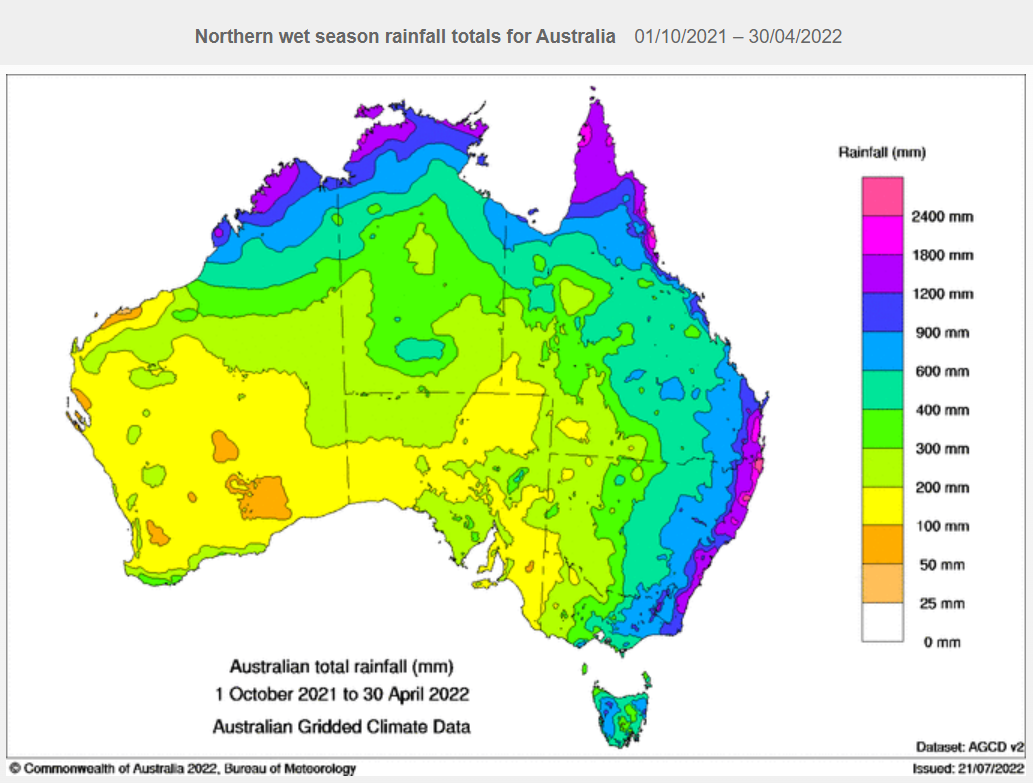
\includegraphics[scale=0.3]{images/bom_2022_wet_season.png}
\caption{Annual rainfall between October 2021 and April 2022.}
\label{fig:rainfall}
\end{figure}
\citep{bom2022}

\subsection{Variability of savanna}
Although the vegetation class of tropical savanna may appear homogeneous within the NT, there is significant variability within its distribution. Tropical savanna is defined as an open woody upper stratum over persistent c4 grasses \citep{williamsetal1997}, with or without a mid stratum of woody shrubs \citep{lehmannetal2011}. The savanna vegetation class of the NT, consists of tall eucalypt dominated woodlands or open woodlands in the coastal and sub-coastal regions, transitioning into low Acacia dominated shrublands, and almost treeless grasslands towards the semi arid southern part of its distribution \citep{foxetal2001, williamsetal1997, woinarski2007}; following  the NT's rainfall gradient \citep{houseHall2001, hutleyetal2011, lehmannetal2011, williams1996}.

In addition to rainfall, soil nutrients affect savanna variability and contribute to patchiness \citep{williams1996}. According to \cite{houseHall2001} low soil fertility within low rainfall regions will generally transition savanna from a semi-arid to an arid vegetation class. Conversely, high soil fertility within high rainfall regions will generally transition savanna woodland into forest \citep{houseHall2001, williams1996}. Therefore, soil variability in conjunction with rainfall increases savanna variability and patchiness within the NT.

In recent decades more emphasis has been placed on fire than climate and/or soil nutrients as a driver of savanna distribution and variability. According to \cite{prioretal2010}, savanna tree recruitment is thought to be subject to a fire-mediated bottleneck, where frequent fire inhibits the transition of a sapling into a mature tree. However, this model was derived from African savanna research, and \cite{murpheyetal2015} disputes the effectiveness of this model within an Australian context. Further stating, that eucalypt dominated Australian savannas avoid the fire trap as their extreme fire tolerance makes them relatively unresponsive to fire, reaching fire resistant size more quickly than other trees \citep{murpheyetal2015}.

Further to this, fire generally acts as a positive feedback, reducing canopy cover, thereby increasing c4 grass production \citep{bondetal2005, bond2008, woinarskietal2004b}, which increases fuel loads and may result in higher fire intensity \citep{lehmannetal2011, ratnametal2011}. Additionally, studies have demonstrated that savanna has transitioned into forest with the removal of fire on multiple continents \citep{bond2008}, including Australia \citep{woinarskietal2004b}. Further to this, fire is known to reduce tree growth and diameter at breast height (DBH) in northern Australian savannas \citep{murphyetal2010, williams1999}, and increase the size of tree hollows which result in less above ground biomass (AGB) \citep{peetersbutler2014}. 

\subsection{Carbon storage}
Due to the global distribution of tropical savannas, they are considered an important carbon (C) sink. According to \cite{Graceetal2006} on average, global savannas store $\sim120 \ tC \ ha^{-1}$ within its vegetation mass and organic soil matter. Although this is less than half that of global tropical forest ($\sim320 \ tC \ ha^{-1}$), it still represents $\sim15 \%$ of global stored C \citep{Graceetal2006}. Within northern Australian tropical savanna, C stock has been measured at $\sim53 \ tC \ ha^{-1}$ \citep{chenetal2002}, which is less than half that of the global average. Even though the two biomes record a similar net primary production NPP, the difference in C stock is primarily the result of frequent fires; returning sequestered C back into the atmosphere \citep{Graceetal2006}. Therefore, even though global and northern Australian tropical savanna store less C than tropical forests, due to their distribution they are still an important C sink.

\subsection{Emissions from land clearing}
Australian tropical savannas (including the NT) remains structurally intact from agriculture and land use change \citep{franklinetal2008, hutleyetal2016, kuttetal2012}. Since clearing controls began in 1999 for zoned and unzoned land tenure \citep{ntplanningact1999}, and 1992 for pastoral lease tenure \citep{ntpastorallandact1992} within the NT; $\sim1974\ km^2$ of tropical savanna has been approved for clearing \citep{unzonedclearing2022, pastoralclearing2022}. Additionally, according to land use mapping undertaken by \cite{landuse2016}, $\sim4563 \ km^2$ of what once was likely considered tropical savanna has undergone land use change or deforestation for agriculture and intense use. However, the total amount of clearing (full felling and selective clearing) within the NT is unknown.

According to \cite{hutleyetal2016}, the total emissions released from clearing native savanna woodland for a site located $\sim300 \ km$ south of Darwin, equated to $148.3 \ Mg\ CO_{2}-e \ ha^{-1}$. Of the total emissions, $82\%$ was released due to the burning of biomass, $10\%$ were attributed to soil disturbance and $8\%$ attributed to debris curing and decay.

\subsection{Quantifying AGB and C extent at a regional scale}
Understanding C sinks and sources within the tropical savanna context is necessary for decision makers and C accounting. However, accurately quantifying C emissions from land use change and fire at a local or regional level is difficult due to lack of existing baseline data \citep{woinarski2007}, financial constraints and structural variability \citep{barrettetal2001, houseHall2001}. Although the NT has a significant store of vegetation, fire scar, land system spatial data, and many remotely sensed products, the NT does not have regional scale AGB mapping.

\subsection{Estimating AGB}
AGB is an important biophysical parameter for understanding the C cycle within a terrestrial context. The most accurate way to estimate biomass is through direct measurements; however, this method is destructive and requires the termination of the tree \citep{clarkkellner2012, luetal2014}. Nonetheless, direct measurements of AGB, often result in the development of allometric models \citep{clarkkellner2012, luetal2014}. Once allometric models have been developed for a region, or vegetation community, stand biomass can be estimated using diameter at breast height (DBH) or DBH in conjunction with tree height biophysical parameters \citep{cooketal2005, williamsetal2005b}, which is non-destructive and data collection is less prohibitive \citep{clarkkellner2012, luetal2014}. However, it is important to note that estimating stand biomass from allometric models may lead to significant uncertainty, due to the fact that soil conditions, rainfall gradients, tree density and land-use history all influence growth rates, which effect tree height and DBH, and therefore estimated AGB (EAGB) \citep{clarkkellner2012}.

\subsection{Scaling up EAGB}
Nonetheless, there are many examples of modeling EAGB from satellite derived surface reflectance (SR) and other modeled products throughout the world \citep{gasparretal2010, lietal2020, wuetal2016, wuetal2022, zhengetal2004}. 
Whereby EAGB (from allometric scaling) is scaled up to remotely sensed data; as only airborne or satellite derived data allows the ability to sample large areas of the required vegetation class or biome \citep{clarkkellner2012}. However, extrapolating relationships between EAGB values with the spectral signatures of SR bands, spectral indices (SI) and/or modeled biophysical vegetation parameters, adds error into the predictions \citep{clarkkellner2012}. Accordingly, it is important to assess the model for accuracy and precision \citep{clarkkellner2012}.

According to \cite{clarkkellner2012}, the distinction between the accuracy and precision of modeled EABG at a regional scale derived from field based EAGB and satellite data is critical. Nonetheless, depending on its use, remotely sensed metrics with unknown accuracy are arguably sufficient for monitoring EAGB and EC stocks within a land type, and therefore, approximate loss of EABG and EC from historic and future land clearing at a regional level. Additionally, such a product could arguably be useful in the monitoring of long term trends in EAGB resulting from burning practice. However, such a product would not contain sufficient accuracy to report on global C accounting budgets or to inform $CO^2$ equivalent emissions for scientific climate change research \citep{clarkkellner2012, wuetal2016}.
\newpage
\section{Research aims and objectives}

\subsection{Research question}
What is the relationship between allometry-derived EAGB and EC, with Landsat derived products and meteorology data within the tropical savanna of the NT?
\subsection{Aim}
This study aims to use a medium resolution remote sensing product together with meteorology data to estimate AGB and/or C across NT tropical savannas. This will be accomplished by assessing if a relationship can be identified between allometry calculated EAGB and Landsat derived products including but not limited to: SR, SI, modeled fractional cover (FC), modeled woody foliage projective cover (WFPC), fire scar mapping (FSM) and modeled canopy height (CH) etc., in conjunction with freely available meteorological data-sets using machine learning.

\subsection{Objectives}
The objectives of this study include:

\begin{enumerate}
    \item To quantify EAGB extent within NT tropical savanna.
    \item To quantify EC within NT tropical savanna.
    \item To investigate relationships between EAGB and EC with Landsat derived SR, SI and modeled biophysical metrics.
    \item To determine which Landsat product parameters or indices yield strongest correlations through principle component analysis (PCA).
    \item To determine how fire interacts with the model and mask out if required.
    \item To develop several machine learning models to predict EAGB and EC extents from Landsat derived parameters.
    \item To assess each of the models accuracy and precision.
    \item To produce a python pipeline that can apply the most precise EAGB and EC extent models to either Landsat seasonal composites or Landsat single date imagery.

\end{enumerate}
\newpage

\section{Methods}
\subsection{Study area}
The proposed study area covers the northern third of the NT. This region is broadly covered by \emph{E. tetrodonta} and \emph{E. miniata} dominated savanna  \citep{foxetal2001, williams1996}. Although there is variability within this vegetation community it is broadly described as having an open overstory ($<50\%$ cover) with an understory of c4 grasses and herbs \citep{bondetal2005, bond2008, foxetal2001, williamsetal1997} with or without a woody midstory \citep{lehmannetal2011}. The vegetation class is recorded as having limited floristic variation within the \emph{E. tetrodonta} and the study area is subject to seasonally dry winters and seasonally wet summers with an annual mean rainfall decreasing from north to south \citep{williams1996}. The average annual rainfall recorded for Darwin Airport, Katherine City Council, Timber Creek, Daly Waters Airstrip and Borrolloola Airport are $1,724 \ mm$, $967 \ mm$, $958 \ mm$, $624 \ mm$  and $902 \ mm$, respectively \citep{bom2022}.
 
 Based on Geographic Information System (GIS) interrogation of land system mapping produced by \cite{lynchetal2012}, the study area is  $\sim390,140 \ km^{2}$ and contains 17 relevant land system classes. Of the 17 classes, the majority of land mass is classified as one of four groups: lateritic plains and rises, sandstone plains and rises, rugged quartz sandstone plateaux and hills and alluvial plains, which cover $\sim12,531.5 \ km^2$, $\sim67,998.77 \ km^2$, $\sim56,490.19 \ km^2$ and $\sim42,141.29 \ km^2$, respectively (Figure \ref{fig:landsystemclass}). Full land systems class descriptions can be found in the draft report "Summary of the Origin and Derivation of the 1:250,000 Land System Descriptions for the Northern Part of the Northern Territory" \citep{lynchetal2012}.
 
\subsection{Sampling design}
Tree basal area for each of the associated historical field sites has been collected using the $1 \ ha$ star transect methodology described by \cite{muiretal2011}. Whereby three $100 \ m$ tapes are run north to south $(0^{\circ}C - 180^{\circ}C)$, northeast to southwest $(60^{\circ}C - 240^{\circ}C)$ and southeast to northwest $(120^{\circ}C - 300^{\circ} C)$ from a central point. Seven species level, basal counts at breast height ($1.3 \ m$) from ground surface using and factor gauge were collected at the $25 \ m, \ 50 \ m$ and $75 \ m$ measurements of the three tapes. Additionally, a site location was collected at the centre point of each site using a hand held global positioning system (GPS).

\begin{figure}[h!]
\label{fig:landsystemclass}
\centering
 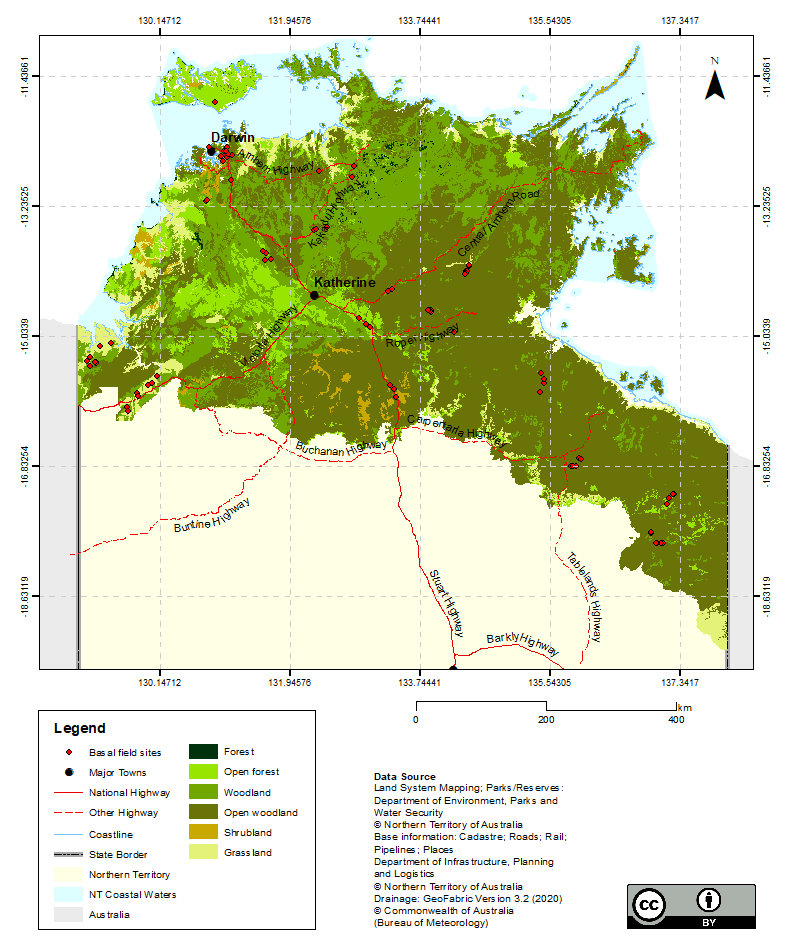
\includegraphics[scale=0.75]{images/savanna.png}
 \caption{Overview of vegetation and land system classes within proposed study area, including current field site locations.}
\end{figure}

\vspace{40cm} %5mm vertical space

\subsection{Data preparation}
\subsubsection{Field data}
The species level basal factor gauge count data used in this study will be compiled from multiple sources and formats. All site location information will be compiled into a single data-frame, and projected to Geocentric Datum of Australia 1994 (GDA94). Following this, species level basal count proportions will be calculated to inform species level, live tree basal area (LTBA) (equation \ref{eq:ltba}) and species level standing tree basal area (STBA) (equation \ref{eq:stba}). 


\begin{equation} \label{eq:ltba}
    LTBA\ = \frac{\sum \ F(L)}{n}
\end{equation}

\begin{equation} \label{eq:stba}
    STBA\ = \frac{\sum \ F(L + D)}{n}
\end{equation}

Where F represents the basal gauge factor, L and D the total live and dead stems per species per site respectively, and n the number of measurement points \citep{muiretal2011}.

\textbf{Note}: LTBA and STBA are calculated in units $m^2 \ ha^{-1}$.

\subsubsection{Calculating EC and EAGB stock}
Species will be reclassified into one of the following groups \emph{E . tetrodonta, E. miniata, Corymbia porrecta, C. bleeseri, Erythrophleum chlorostachys and Terminalia ferdinandiana}, where all species not listed will be classified as \emph{T. ferdinandiana}, and the EC stock coefficients will be applied in accordance with the methodology described in \cite{cooketal2005}. In addition to this, EC stock for leaves, twigs, bark, wood, branches, stems and EAGB (kg) will be calculated \citep{cooketal2005} from LTBA and STBA. Following this, extant carbon mass will be converted to extant biomass using the co-factors 0.47 for foliage and 0.49 for all other parts \citep{cooketal2005, gifford2000} (equation \ref{eq:agb}).

\begin{equation}\label{eq:agb}
    EAGB\ = \frac{\sum{(C_{leaves}))}}{0.47} + \frac{\sum{(C_{twigs}, C_{bark}, C_{wood}, C_{branches}, C_{stems})}}{0.49}
\end{equation}

Where C represents the EC extent stored within each of the woody vegetation parts.

% --------------------------------------------- Remote sensing -----------------------------------------

\subsection{Remotely sensed products}
\subsubsection{Landsat data}
The Landsat satellite data capture program is the longest continuous earth observation program in the world, with the first satellite launch in 1972 \citep{stabenetal2018}. Landsat satellites are fitted with multi band sensors which capture radiance data at a range of wavelengths which include but are not limited to the visible bands (red, green and blue), and near-infrared (NIR) \citep{Storey2014}. In addition to this, Landsat satellites revisit the same location every 16 days, which makes this data ideal for monitoring and mapping land cover and woody vegetation at a regional scale \citep{slats2015_16, Armstrongetal.2009, stabenetal2018}. Additionally, spectral mixture analysis has consistently been demonstrated to improve estimates of vegetation biophysical information including biomass \citep{peddleetal2001}. Accordingly, Landsat SR and modeled remote sensing products are temporally, spatially and financially ideal for this study.

\subsubsection{Landsat data corrections}
All Landsat SR data will be obtained through the QLD government's, Remote Sensing Centre (RSC), and will have undergone the following corrections:
\begin{enumerate}
    \item Landsat radiance data will be geometrically corrected by the United States Geological Survey (USGS), before being downloaded by the RSC.
    \item Landsat radiance data will be converted to SR and masked using the methodology outlined in \cite{floodetal2013}.
    \item Differences between Landsat sensors (TM, ETM+ and OLI) SR data will be corrected for cross platform anomalies using the methodology outlined in \cite{flood2014}.
\end{enumerate}

\subsubsection{Surface reflectance}
SR data, seasonal composites and single date imagery will be assessed for suitability. In the first instance, dry season (1 May until 30 September) and annual SR composites will be assessed, following this, single date SR may also be included. Seasonal composites are a multi-band image, whereby each resulting band contains pixel values that mathematically represent the average residual value for the season and have been produced using the methodology described by \cite{flood2013}. SI will also be calculated in accordance with the SI equations outlined in Table \ref{table:si}.

%\begin{landscape}

{\renewcommand{\arraystretch}{2}%
\begin{sidewaystable}[]%h!]
\caption{List of the SI calculations that will be performed on the SR bands values and applied to the modelling. Table has been reproduced from \cite{staben2016}}
\label{table:si}
\centering

%\begin{tabular*}{\textheight}{c @{\extracolsep{\fill}} c c c}

%\begin{tabular}{c c c} 
\begin{tabular*}{\textwidth}{c @{\extracolsep{\fill}} c c c}
 \hline
Spectral Index & Formula & Reference \\[1ex] 
 \hline
 Normalised Difference Vegetation Index & $NDVI\ = \frac{\rho_{NIR} - \rho_{Red}}{\rho_{NIR} + \rho_{Red}}$ & \citep{tucker1979}  \\ 
 Green Soil Adjusted Index & $GSAVI\ = \frac{\rho_{NIR} - \rho_{Green}}{\rho_{NIR} + \rho_{Green} + L} * (1 + L)$ &  \citep{sripada2006} \\ 
  Green Normalised Difference Vegetation Index & $GNDVI\ = \frac{\rho_{NIR} - \rho_{Green}}{\rho_{NIR} + \rho_{Green}}$ & \citep{bushnagel1993} \\ 
 Chlorophyll Vegetation Index & $CVI = \frac{\rho_{NIR}}{\rho_{Green}} \times \frac{\rho_{Red}}{\rho_{Green}}$ & \citep{vincini2008} \\ 
 Normalised Difference Greenness Index & $NDGI = \frac{\rho_{Green} - \rho_{Red}}{\rho_{Green} + \rho_{Red}}$ & \citep{bannarietal1995} \\
 Normalised Burn Ratio SWIR2 & $NBR = \frac{\rho_{NIR} - \rho_{SWIR2}}{\rho_{NIR} + \rho_{SWIR2}}$ & \citep{leietal2011} \\
  Normalised Burn Ratio SWIR1 & $NDII = \frac{\rho_{NIR} - \rho_{SWIR1}}{\rho_{NIR} + \rho_{SWIR1}}$ & \citep{leietal2011} \\
  Green Difference Vegetaion Index & $GDVI = \rho_{NIR} - \rho_{Green}$ & \citep{sripada2006} \\
  Modified Soil Adjusted Vegetion Index & $MSAVI = \frac{2 \times \rho_{NIR} + 1 - \sqrt{(2 \times \rho_{NIR} + 1)^{2} -8 \times (\rho_{NIR} - \rho_{Red}))}}{2}$ & \citep{qietal1994} \\
  Difference Vegetation Index & $DVI\ = NIR - Red$ & \citep{tucker1979} \\
  Soil Adjusted Vegetation Index & $SAVI\ = \frac{\rho_{NIR} - \rho_{Red}}{\rho_{NIR} + \rho_{Red} + L} * (1 + L)$ & \citep{huete1988} \\[2ex]
  Modified Simple Ratio & $MSR\ = \frac{\frac{\rho_{NIR}}{\rho_{Red}} - 1}{\sqrt{\frac{\rho_{NIR}}{\rho_{Red}}} + 1}$ & \citep{chen1996} \\[2ex] 
 \hline
%\end{tabular*}
\end{tabular*}
\end{sidewaystable}
}

%\end{landscape}

\subsubsection{Modeled products}

In addition to Landsat SR data the following modeled remote sensing products will be assessed for model parameterisation:

\begin{enumerate}

    \item Seasonal and single date FC product  - developed through the RSC and collaborative partners \citep{tindaletal2012}. The FC product was developed using a linear spectral unmixing model with all available Landsat TM/ETM+ imagery and field based site data \citep{tindaletal2012}. The FC product contains seasonal or daily percentage  measures of photosynthetic, non-photosynthetic and bare ground land cover fractions \citep{tindalletal.2014, qldseasonalfc2022}.
    \item Annual modeled woody foliage projective cover (WFPC) product - developed by  \cite{staben2016} is medium resolution ($30\ m \times \ 30 \ m$) nearest neighbour classification derived from field measured (WFPC) and high resolution aerial photography.
    \item Annual canopy height (CH) product - developed by  \cite{stabenetal2018} is medium resolution ($30 \ m \times \ 30 \ m$) $99 \ th$ percentile model derived from LiDAR and Landsat imagery using a random forest regression model.

\end{enumerate}

In addition to Landsat derived SR and remotely sensed products, the following meteorological data may be assessed for suitability:

\subsubsection{Meteorological data}
Due to the fact that tropical savanna AGB, distribution and variability are correlated with climate, the following freely available meteorological data-sets will be assessed for parameter suitability. The data-sets will be obtained from SILO database hosted by the QLD government, and were constructed from observational records collated from the Bureau of Meteorology (BOM), and other providers. All available variable specific records on a daily or monthly temporal scale have been concatenated from approximately $4,600$ locations across Australia. These point data-sets have then been spatially interpolated into variable specific $0.05^{\circ}$ Australia wide gridded data-sets. Missing observation data is patched with interpolated estimates, and missing patches have been filled with longer term averages \citep{jeffreyetal2001}.

Annual compilations of all meteorological data will be downloaded as NetCDF files and projected to the Geocentric Datum of Australia 1994 in the Cartesian 3D CS (geocentric) coordinate system (epsg: 4938). Each variable will then be exported as a single date grey-scale geo-tiff, in accordance with its metadata and temporal extent (daily, monthly or annual). Following this, the specific meteorological variables (see Table. \ref{table:qld_gridded_data}) will be assessed for model parameterisation \citep{silo2022}.

%\begin{landscape}

\begin{table}[]%h!]
\caption{List of the meteorological variables that will be tested within the model. Data obtained from \cite{silo2022}, accessed on 1 September 2022}
\label{table:qld_gridded_data}
\centering
%\begin{tabular}{c c c} 
\begin{tabular*}{\textwidth}{c @{\extracolsep{\fill}} c c c}
 \hline
 Abbreviation & Variable & Unit \\ [0.5ex] 
 \hline\hline
 daily rain & Daily rainfall & $mm/day$  \\ 
  et morton actual & Mortons estimate of areal actual evapotranspiration & $mm/day$ \\ 
%   et morton potential & Mortons estimate of potential evapotranspiration & $mm$ \\ 
%   et morton wet & Mortons estimate of wet-environment areal evapotranspiration over land & $mm$ \\ 
%   et short crop & FAO56 estimate of short crop potential evapotranspiration & $mm$ \\ 
%   et tall crop & ASCE estimate of tall crop potential evapotranspiration & $mm$ \\ 
%   evap pan & Class A pan evaporation & $mm$ \\ 
  %evap\_morton\_lake & Mortons estimate of shallow lake evaporation & mm \\ 
%   evap syn & Synthetic estimate of class A pan evaporation & $mm$ \\ 
  max temp & Maximum temperature & $^{\circ} C/day$ \\ 
  min temp & Minimum temperature & $^{\circ} C/day$ \\ 
%  monthly rain & Monthly rainfall & $mm$  \\
%  mslp & Mean sea level pressure & $hPa$ \\
 radiation & Solar radiation - total incoming downward shortwave radiation & $MJ/m^{2}/day$ \\ 
 rh tmax & Relative humidity at the time of maximum temperature & $\%/day$ \\
 rh tmin & Relative humidity at the time of minimum temperature & $\%/day$ \\
%  vp & Vapour pressure & $hPa$ \\
% vp deficit & Vapour pressure deficit at mean temperature, $T = Tmin + 0.75 \times (Tmax-Tmin)$ & $hPa$  \\
 [1ex] 
 \hline
\end{tabular*}
\raggedright
\end{table}


%\end{landscape}

\textbf{Note}: Due to the low resolution of the meteorological data $0.05^{\circ}$ or $5 \ km$ it is likely that this data will reduce the proposed output resolution. This will occur if the machine learning algorithm places greater importance on one or more of the meteorological variables over that of the medium resolution Landsat data ($30 \ m \times 30 \ m$).

\textbf{Note}: Additional data-sets and SI's may be used which have not been mentioned within this study proposal.

\subsection{Model development}
Data will be processed using a variety of machine learning models. Each model will be implemented using python programming language including the following python modules: Scikit-learn \citep{sklearn2011}, Keras \citep{Korstanje2021} and Py-earth \citep{pyearth2013}.

A selection of four machine learning models will be assessed for suitability:
\begin{itemize}
    \item Random forest (RF) regression
    \item Multiple linear regression (MLR)
    \item Multivariate adaptive regression spline (MARS)
    \item Artificial neural networks (ANN).
\end{itemize}

\textbf{Note}: Final model selection has not been determined at the time of writing this proposal and is subject to change.

\subsubsection{Random forest}
RF regression is an extension of a decision tree (DT) regression. Where a DT algorithm utilises a single tree, RF utilises a user determined quantity of DT's; where each tree is created through random sampling \citep{Armstrongetal.2009, wuetal2022}. As such, the RF model can be created with hundreds of DT models, each model fitted with slightly different data. \citep{Korstanje2021}. Noting that, where machine models can be inaccurate, the average prediction of a large number of DT's is less likely to be inaccurate \citep{Korstanje2021, wuetal2022}.

\subsubsection{Multiple linear regression}
MLR is a statistical method that determines a relationship with each of the independent variables to the dependent variable; the model minimises the sum of squared error \citep{wuetal2022}.

\subsubsection{Multivariate adaptive regression spline}
MARS is a non-parametric algorithm designed for nonlinear problems \citep{wuetal2022}. MARS was developed by \cite{friedman1991}, and determines regression slopes between each of the independent variables with  the dependent variable. MARS interactively adds cut-points "knots" within the data and calculates linear regression equations for the data between each knot until a threshold  of residual error has been reached for all data (forward selection); then due to potential over-fitting removes the knots with high complexity which will be unlikely to effectively predict unseen data (backwards fitting) \citep{wuetal2022}.

\subsubsection{Artificial neural networks}
ANN are intended to simulate the working neurons of the human brain \citep{wuetal2022}. ANN consists of a single input layer and a single output layer with multiple hidden layers. Neurons exist within each layer, and each neuron has an activation function which introduces linear and non-linearity into relationships. Each connection between neurons has a weighted value \citep{wuetal2022}.


\subsubsection{Model development}
During the development of each model, the following concepts will be assessed:

\begin{itemize}

    \item identification and removal of outliers
    \item PCA - the creation of new features based on the combination of strongly correlated features (i.e. humidity and rainfall).
    \item feature importance assessment
    \item hyperparameter tuning of the model.
\end{itemize}

\subsubsection{Model validation}
A five fold cross-validation (CV) method will be used to assess model performance with the machine learning models previously outlined. The CV will be implemented by randomly splitting the data into training ($80\%$) and testing ($20\%$) data-sets, and the machine learning model used will be determined by the following model performance matrices: 

\begin{itemize}

    \item Mean Square Error (MSE) calculates the average of squared errors between actual and predicted values. The MSE is an error metric. As such the smaller the error the better the performance. MSE is not an accuracy metric due to a lack of scale (no fixed scale and no upper bounds). \citep{Korstanje2021}.
    
    \item Root Mean Square Error (RMSE) calculates the squared root of the MSE. The RMSE does not provide any new information relating to model performance, except that it is more intuitive as the error value is returned at the same scale of the variables. Like the MSE, the same data must be compared. \citep{Korstanje2021}.
    
    \item Mean Absolute Error (MAE) calculates the absolute difference between each actual and modeled value, then averages the differences. Interpreting MAE is comparable to interpreting RMSE. \citep{Korstanje2021}.
    
    \item R squared ($R^{2}$) or coefficient of determination is a performance metric generally returning a value between 0 and 1, with 0 indicating a poor model and 1 indicating a perfect model.
    %(equation \ref{eq:r2}).
    \citep{Korstanje2021}.
\end{itemize}

% \begin{equation} \label{eq:mse}
%     MSE = \frac{1}{n} \sum_{} (x_i-y_i)^2
% \end{equation}

% \begin{equation} \label{eq:rmse}
%     RMSE = \sqrt{MSE}
% \end{equation}

% \begin{equation} \label{eq:mae}
% MAE = \frac{1}{n} \sum |x_i-\widehat{y}_i|
% \end{equation}

% \begin{equation} \label{eq:r2}
% R^{2} = 1 - \frac{\sum(x_i-\widehat{y}_i)^2}{\sum(x_i-\overline{y}_i)^2}
% \end{equation}


% Where n represents the sample size, $x_i$, the actual target value and $y_i$, the predicted value \citep{Korstanje2021}.
\newpage

\section{Ethics}
\subsection{Ethical requirements}

\begin{itemize}
\item No human or animal ethical concerns have been identified for this study.
\end{itemize}


\subsection{Legal and intellectual property requirements}
Intellectual property requirements have been identified and are as follows:

\begin{itemize}

\item Historical basal site data under the custodianship of Department of Environment Parks and Water Security (DEPWS) will be used, the Executive Director of Rangelands Division (DEPWS) has approved the use of this data providing that appropriate citation is incorporated.

  \item Products derived from Landsat data by the Joint Remote Sensing Research Program (JRSRP), RSC and RSU will be used, these data-sets are publicly available; as such, no approvals are required to use these products providing that appropriate citations are incorporated.
  
  \item WFPC product derived by Dr. Grant Staben will be used \citep{stabenetal2018}, Dr. Staben has approved the use of this published model providing that the appropriate citation is incorporated.

  \item CH product derived by Dr. Grant Staben will be used \citep{staben2016}, Dr. Staben has approved the use of this published model product providing that the the appropriate citation is incorporated.
  
  \item Some python scripts have been derived by the Remote Sensing Unit, Rangelands Division (DEPWS). All scripts contain an MIT License agreement, allowing for use the scripts without restriction, product providing that appropriate citation are incorporated.
  
  
\end{itemize}
\newpage
%\chapter{Required Resources}
%\addcontentsline{toc}{chapter}{Required Resources}
\section{Resources}
The following resources have been identified in order of relevance to achieve the proposed research aims and objectives:

\begin{enumerate}

\item Access to NTG basal wedge historical data.

\item Access to the QLD RSC's super computer for processing, masking and downloading of required Landsat derived data (surface reflectance, FC etc.) which correspond to historical basal point data.
  
\item Access to Grant Staben's Landsat derived CH model \cite{stabenetal2018}, and WFPC algorithm \cite{staben2016}.
  
\item Storage space on the NTG's remote server (PGB-BAS14) to store, process and analyses approximately ($100 \ - \ 150 \ GB$) of data.

\item Access to field equipment to collect additional basal counts where required. 

\end{enumerate}
\newpage
\section{Timeline}
\subsection{Year one}
\subsubsection{Semester one}
An overview of the proposed tasks and expected completion dates for semester one, year one are outlined in Table \ref{table:sem1y1}.

\begin{table}[h!]
\caption{Timeline for semester one, year one.}
\label{table:sem1y1}
\centering
\begin{tabular*}{\textwidth}{c @{\extracolsep{\fill}} c c c c}
%\begin{tabular}{c c c c} 
 \hline
 Item & Sections & Final Draft  & Submit Date \\ [0.5ex] 
 \hline%\hline
  % Supervision agreement
  Supervision agreement & & Friday week 2 & Friday week 6\\ 
 \hline
 
  % Research Proposal 4-6 pages
 Proposal  & Aims and Objectives & Friday week 2 & Friday week 6 \\ 
     & Resources required & Friday week 2 &  \\ 
     & Proposed timeline & Friday week 2 &  \\ 
     & Permits required & Friday week 2 &  \\ 
     & Methodology & Friday week 5 &  \\ 
    & Background & Friday week 5 &  \\ 
     & References & Friday week 5 &  \\ 
 \hline
 
% Research Proposal Seminar
 Proposal Seminar  & PowerPoint template & Friday week 7 &  Weeks 7-12\\ 
     & Overview & Friday week 7 &  \\
     & Slides & Friday week 8 &  \\
     & Presentation notes & Friday week 9 &  \\ 
 \hline
 Thesis & Methodology &  Friday week 12 & Ongoing\\ 
 & Python Pipeline &  Friday week 10 & \\ 
 & Model Assessment &  Friday week 12 & \\ 
  & Background &  Ongoing & \\  [1ex]
 \hline

\end{tabular*}
\end{table}

\subsubsection{Semester two}
An overview of the proposed tasks and expected completion dates for semester two, year one are outlined in Table \ref{table:sem2y1}.

\begin{table}[h!]
\caption{Timeline for semester two, year one.}
\label{table:sem2y1}
\centering
\begin{tabular*}{\textwidth}{c @{\extracolsep{\fill}} c c c c}
%\begin{tabular}{c c c c} 
 \hline
 Unit & Assessment & Final Draft  & Submit Date \\ [0.5ex] 
 \hline
 
 % SID403 
 SID403 & Analysis plan & n.d. & \\ 
 & Research Writing essay & n.d.  & \\ 
 & Research Presentation & Friday Week 11  & Friday Week 12 \\ 
 \hline
 ENV511 & Essay & n.d. & \\ 
 & Statistical problems & n.d.  & \\ 
 & Project Report & Friday Week 11  & Friday Week 12 \\ [1ex]
 \hline
\end{tabular*}
\end{table}

% -------------------------------------------------- Year 2 --------------------------------------------------------
\newpage
\subsection{Year two}
\subsubsection{Semester one}
An overview of the proposed tasks and expected completion dates for semester one, year two are outlined in Table \ref{table:sem1y2}.


\begin{table}[h!]
\caption{Timeline for semester one, year two.}
\label{table:sem1y2}
\centering
\begin{tabular*}{\textwidth}{c @{\extracolsep{\fill}} c c c c}
 \hline
 Item & Sections & Final Draft  & Submit Date \\ [0.5ex] 
 \hline
 
 % Thesis 
 Thesis  & Data analysis &  Friday week 4 & Ongoing\\ 
 & Discussion &  Friday week 12 & \\ 
 & Introduction &  Ongoing & \\ 
 & Results &  Friday week 12 & \\ [1ex]
 \hline
\end{tabular*}
\end{table}


\subsubsection{Semester two}
An overview of the proposed tasks and expected completion dates for semester two, year two are outlined in Table \ref{table:sem2y2}.
\begin{table}[h!]
\caption{Timeline for semester two, year two.}
\label{table:sem2y2}
\centering
\begin{tabular*}{\textwidth}{c @{\extracolsep{\fill}} c c c c}

 \hline
 Item & Sections & Final Draft  & Submit Date \\ [0.5ex] 
 \hline
 % Thesis 
 Thesis & Recommendations &  Friday week 3 & Monday week 15\\ 
 & Maps/Figures &  Friday week 5 & \\ 
 & Abstract &  Friday week 6 & \\ 
 & Appendices &  Friday week 8 & \\ 
 & References &  Friday week 9 & \\ 
 & Final Draft &  Friday week 11 & \\
% Results Seminar
 \hline
  Results Seminar  & Overview & Friday week 6 & Weeks 9-11 \\ 
  & Slides & Friday week 8 &  \\ 
  & Notes & Friday week 9 &  \\[1ex]
  \hline
\end{tabular*}
\end{table}





\medskip
\newpage
\bibliography{references}
}
%\end{flushleft}
\end{document}
